\chapter{Dilema do prisioneiro hiper-racional}

No início deste trabalho nós introduzimos o Dilema do Prisioneiro com matriz de pagamentos \ref{mpdp} e vimos que o perfil de estratégias $\{\textit{delação},\textit{delação}\}$ era o único equilíbrio de Nash do jogo. Agora vamos considerar o mesmo jogo, com a mesma matriz de pagamentos, porém com $v_1$ e $v_2$ como jogadores hiper-racionais.

Como nesse jogo temos apenas dois jogadores e duas estratégias podemos denotar a matriz de preferências dos jogadores como

\begin{equation}
    \label{matrizPrefPD}
    \mathcal{R}=
    \begin{bmatrix}
        r_1 & 1-r_1\\ 
        1-r_2 & r_2 
    \end{bmatrix}
\end{equation}
onde $r_1,r_2\in[0,1]$ denotam a preferência do jogador por si mesmo. Vamos desconsiderar valores negativos para as preferências nesse jogo, pois o pagamento virtual da estratégia $\textit{delação}$ aumenta quando um jogador tem preferência negativa pelo outro, somente reforçando a dominância do jogo clássico, e o pagamento virtual da estratégia $\textit{silêncio}$ se torna dominante quando um jogador tem preferência negativa por si mesmo. 

Denotaremos a probabilidade do jogador $i=1,2$ usar a estratégia $\textit{silêncio}$ por $x_{i,s}$ e a estratégia $\textit{delação}$ por $x_{i,d}=(1-x_{i,s})$. Assim, sendo $j$ o adversário de $i$, a equação de replicação para esse jogo é dada por
\begin{equation}
\begin{split}
    \label{eqRepPDHREx}
    \dot{x}_{i,s}&= \!\begin{multlined}[t]
    x_{i,s}(1-x_{i,s})\left\{x_{j,s}\left[r_i(-2)+(1-r_i)(5)\right]\right.\\
    + \left. (1-x_{j,s})\left[r_i(-2)+(1-r_i)(5)\right] \right\}
    \end{multlined} \\
    &= x_{i,s}(1-x_{i,s})\left[ r_i(-2)+(1-r_i)(5) \right] \\
    &= x_{i,s}(1-x_{i,s})\left[ 5-7r_i \right]
\end{split}
\end{equation}

Note que a variação nas probabilidades de $i$ dependem somente de suas hiperpreferências, sendo completamente independente do perfil de estratégias do seu adversário. De fato, para valores de $r_i$ maiores que $\frac{5}{7}$ o jogador $i$ irá, eventualmente, sempre escolher $\textit{delação}$, para valores menores que $\frac{5}{7}$ irá sempre escolher $\textit{silêncio}$ e para valores iguais à $\frac{5}{7}$ o estado inicial de $i$ será seu estado de hiperequilíbrio. Esse comportamento pode ser observado na figura \ref{fig:pd-neg-payoff}.

\begin{figure}[h]
    \caption{Probabilidade do jogador usar \textit{silêncio}, onde a condição inicial é 0.5 para todas estratégias para ambos jogadores.}
    \centerline{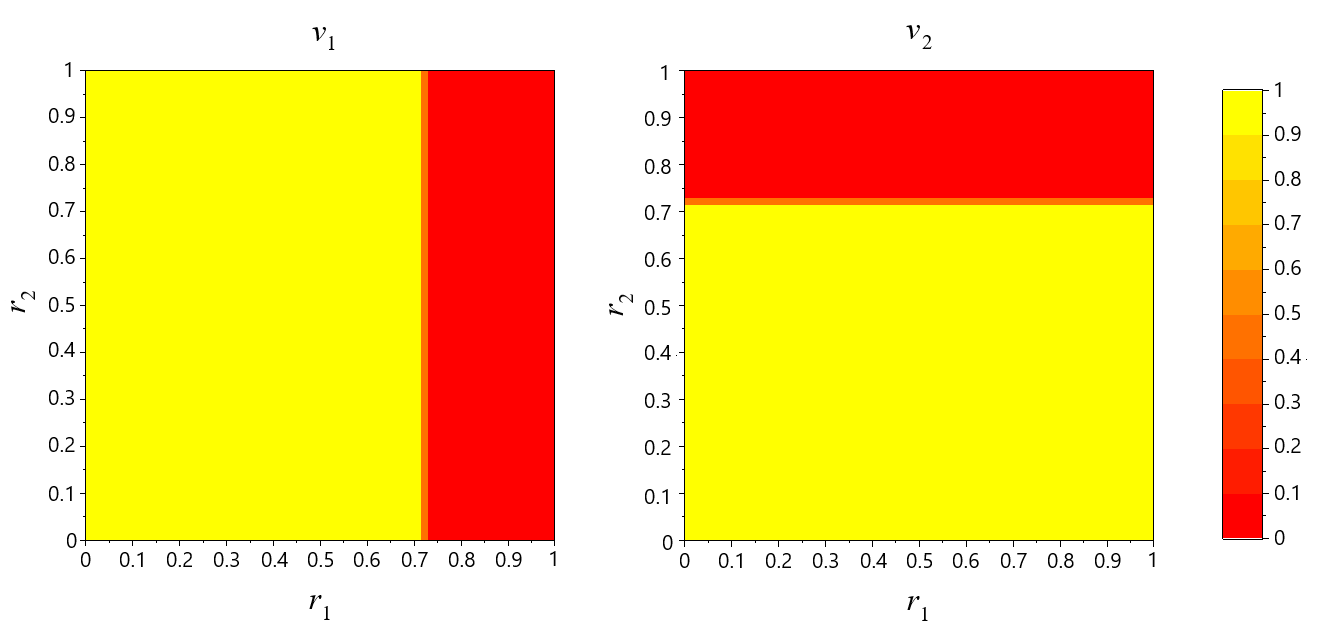
\includegraphics[scale=0.43]{./img/PD-neg-payoff.png}}
    \label{fig:pd-neg-payoff}
\end{figure}

Nos interessa saber se esse comportamento é geral ou uma exceção e, por isso, vamos usar um definição mais geral para o pagamento do dilema do prisioneiro, dada por
\begin{equation}
    \label{payoffGeralPD}
    B=
    \begin{bmatrix}
        R & S\\ 
        T & P 
    \end{bmatrix}
\end{equation}
onde $R$ é a recompensa pela cooperação entre os jogadores, $T$ é a tentação para trair, $P$ é a punição pela traição mútua e $S$ é o pagamento do ingênuo, que foi traído. Para que esses valores representem um dilema do prisioneiro eles devem respeitar a seguinte restrição.

\begin{equation}
    \label{desigualdadePD}
    T>R>P>S
\end{equation}

Assim, a equação de replicação para um dilema do prisioneiro geral é dada por

\begin{equation}
\begin{split}
    \label{eqRepPDGeral}
    \dot{x}_{i,s}&= \!\begin{multlined}[t]
        x_{i,s}(1-x_{i,s})\left\{x_{j,s}\left[r_i(R-T)+(1-r_i)(R-S) \right] \right.\\
        + \left. (1-x_{j,s})\left[r_i(S-P)+(1-r_i)(T-P)\right] \right\}
    \end{multlined} \\
    &= \!\begin{multlined}[t]
    x_{i,s}(1-x_{i,s})\left\{r_i \left[x_{j,s}(R-T)+(1-x_{j,s})(S-P) \right] \right. \\
    + \left. (1-r_i)\left[ x_{j,s}(R-S) + (1-x_{j,s})(T-P)\right] \right\}
    \end{multlined}
\end{split}
\end{equation}

Um jogador não muda sua estratégia quando $\dot{x}_{i,s}=0$. Portanto, vamos assumir que $\dot{x}_{i,s}=0$ para algum perfil de estratégias $\BS{X}$ e, assim, a equação $\eqref{eqRepPDGeral}$ se torna
\begin{equation}
    0 = \!\begin{multlined}[t]
        r_i \left[x_{j,s}(R-T)+(1-x_{j,s})(S-P) \right] \\
    + (1-r_i)\left[ x_{j,s}(R-S) + (1-x_{j,s})(T-P)\right]
    \end{multlined}
\end{equation}
que podemos simplificar da para obtermos
\begin{equation}
    0 = r_i(S-T) + x_{j,s}(R-S) + (1-x_{j,s})(T-P)
\end{equation}
e, por fim, isolamos $r_i$ para obter
\begin{equation}
    \label{rSela}
    r_i=\frac{x_{j,s}(T+S-P-R)+P-T}{S-T}
\end{equation}

Com isso, se a igualdade 
\begin{equation}
    \label{condicaoIndependencia}
    T+S-P-R = 0
\end{equation}
for satisfeita, basta que tenhamos
\begin{equation}
    r_i=\frac{P-T}{S-T}
\end{equation}
para que $\dot{x}_{i,s}=0$ para todo $t>0$, fazendo com que a condição inicial de $i$ seja um hiperequilíbrio. Note que a igualdade $\eqref{condicaoIndependencia}$ é, de fato, satisfeita para os pagamentos de \ref{mpdp}, $R=-2,S=-7,T=0,P=-5$. Além disso, a igualdade $\eqref{rSela}$ nos dá uma forma de encontrar o ponto de sela, onde qualquer variação em $r_i$, para mais ou para menos, vai alterar o resultado do jogo. Também podemos ver uma ligação entre $r_i$ e $x_{j,s}$, que iremos avaliar agora.

Podemos alterar a matriz \ref{mpdp} para que haja uma dependência diretamente proporcional entre $r_i$ e $x_{j,s}$, basta tomar $R=-1$, assim a equação $\eqref{rSela}$ se torna
\begin{equation}
    r_i=\frac{5+x_{j,s}}{7}
\end{equation}

Como $x_{j,s}\in[0,1]$, para valores de $r_i$ no intervalo $[\frac{5}{7},\frac{6}{7}]$ a distribuição de estratégias do jogador $i$ depende diretamente da distribuição de $j$ e, em algumas condições especiais, temos um ponto de equilíbrio interno para cada um desses valores de $r_i$. Discutiremos mais sobre esse ponto de equilíbrio ao final desta seção. Como a matriz de pagamentos é igual para ambos jogadores, esse intervalo de dependência é igual para os dois jogadores e a solução dentro do quadrado $[\frac{5}{7},\frac{6}{7}]\times[\frac{5}{7},\frac{6}{7}]$ dependerá da distribuição de estratégias de ambos. Esse comportamento pode ser observado na figura \ref{fig:pd-neg-payoff-dependant}, onde o ponto de sela da solução se encontra na diagonal do quadrado $[\frac{5}{7},\frac{6}{7}]\times[\frac{5}{7},\frac{6}{7}]$. Também é interessante notar que a estratégia $\textit{silêncio}$ é predominante no nosso gráfico, pois $\textit{delação}$ só é vantajoso para de $r_i$ próximos de $1$.

\begin{figure}[h]
    \caption{Probabilidade do jogador usar \textit{silêncio} ao tomar $R=-1$ no pagamento dado por \ref{mpdp}, onde a condição inicial é 0.5 para todas estratégias para ambos jogadores.}
    \centerline{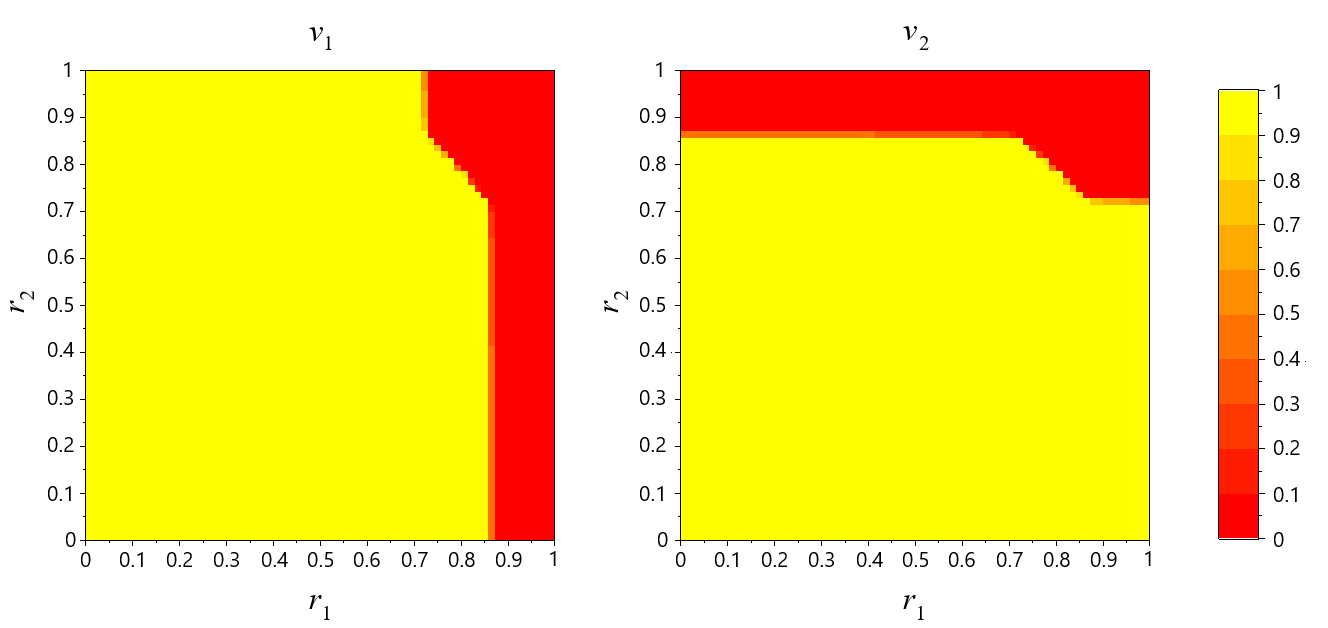
\includegraphics[scale=0.43]{./img/PD-neg-payoff-dependant.png}}
    \label{fig:pd-neg-payoff-dependant}
\end{figure}

Da mesma maneira, podemos novamente usar o pagamento definido em \ref{mpdp} e tomar $S=-6$ para que haja uma dependência inversamente proporcional entre $r_i$ e $x_{j,s}$, assim a equação $\eqref{rSela}$ se torna
\begin{equation}
    \label{eqQuadradoEx}
    r_i=\frac{5-x_{j,s}}{6}
\end{equation}

Agora temos $[\frac{4}{6},\frac{5}{6}]$ como nosso intervalo de dependência que, novamente, é igual para ambos jogadores. Agora o ponto de sela estará na diagonal do quadrado $[\frac{4}{6},\frac{5}{6}]\times[\frac{4}{6},\frac{5}{6}]$ e, apesar de ainda não ser predominante, a faixa na qual $\textit{delação}$ se torna mais vantajosa aumentou consideravelmente.

\begin{figure}[h]
    \caption{Probabilidade do jogador usar \textit{silêncio} ao tomar $S=-6$ no pagamento dado por \ref{mpdp}, onde a condição inicial é 0.5 para todas estratégias para ambos jogadores.}
    \centerline{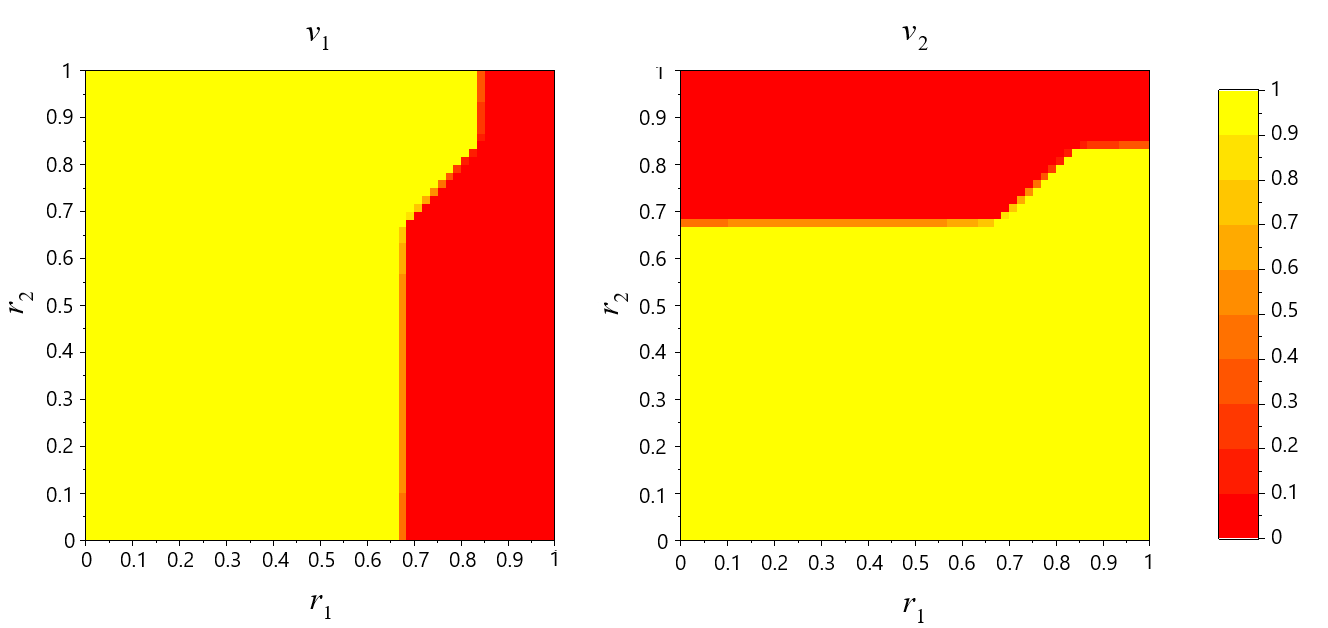
\includegraphics[scale=0.43]{./img/PD-neg-payoff-inverse-dep.png}}
    \label{fig:pd-neg-payoff-inverse-dep}
\end{figure}

A hiper-racionalidade dos jogadores envolvidos faz com que a estratégia $\textit{silêncio}$ se torne, em geral, mais atraente para o jogador mesmo que a condição inicial não esteja muito próxima de $\textit{silêncio}$, enquanto jogadores racionais, mesmo em redes, tendem a preferir $\textit{delação}$ se houver algum vizinho delator \cite{madeo2015}.

Na figura \ref{fig:sobreposicao} temos a sobreposição dos gráficos dos dois jogadores para cada pagamento discutido acima. Assim, podemos ver o resultado do jogo em cada uma das faixas de $r_i$ analisadas anteriormente, explicitando a predominância da estratégia $\textit{silêncio}$ e o fato de que, em muitos casos, um jogador recebe o pagamento do ingênuo $S$, mesmo podendo aumentar seu pagamento efetivo trocando sua estratégia para $\textit{delação}$.

\begin{figure}[h]
    \caption{Sobreposição dos resultados do Dilema do Prisioneiro para cada pagamento apresentado anteriormente. Nos parênteses temos, respectivamente, o resultado do jogador $v_1$ e $v_2$, com $s$ para $\textit{silêncio}$ e $d$ para $\textit{delação}$.}
    \centerline{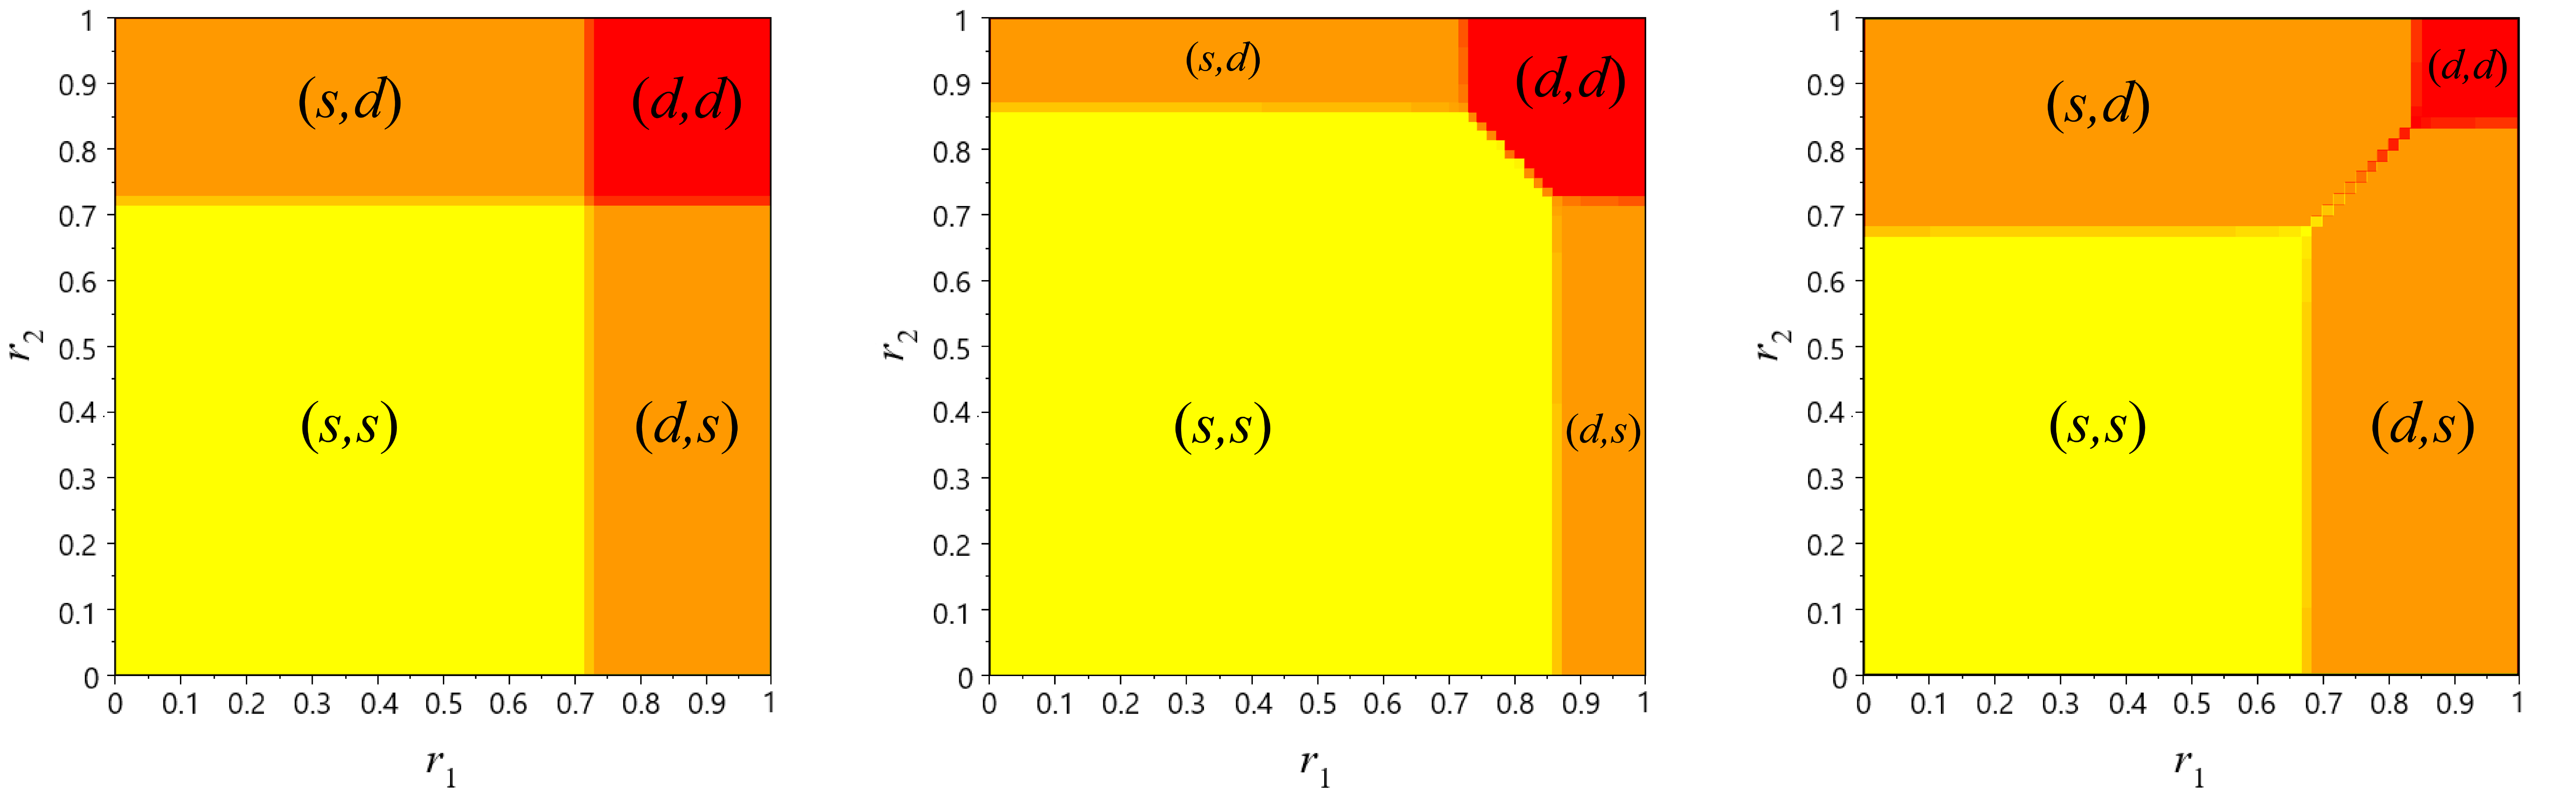
\includegraphics[scale=0.0775]{./img/sobreposicao.png}}
    \label{fig:sobreposicao}
\end{figure}

Essa sobreposição nada mais é do que a soma das probabilidades de $v_1$ e $v_2$ dividida por $2$ exibida na mesma escala das demais figuras desta seção. Assim, as faixas de transição em $\frac{5}{7}$ e nas diagonais dos quadrados $[\frac{5}{7},\frac{6}{7}]\times[\frac{5}{7},\frac{6}{7}]$ e $[\frac{4}{6},\frac{5}{6}]\times[\frac{4}{6},\frac{5}{6}]$ exibem a cor que representa essa média das probabilidades.

Agora iremos analisar a existência dos pontos de equilíbrio interno no interior dos quadrados $[\frac{5}{7},\frac{6}{7}]\times[\frac{5}{7},\frac{6}{7}]$ e $[\frac{4}{6},\frac{5}{6}]\times[\frac{4}{6},\frac{5}{6}]$. Note que podemos reescrever a expressão $\eqref{rSela}$ da seguinte maneira.

\begin{equation}
    x_{j,s}=\frac{r_i(S-T)-P+T}{T+S-P-R}
\end{equation}

Essa expressão nos dá um valor de $x_{j,s}$ em função de $r_i$. Como $j$ não tem conhecimento sobre o valor de $r_i$, esse equilíbrio só existe quando $r_i=r_j$, pois nessas condições teremos a expressão

\begin{equation}
    \label{eqInternoPDHR}
    x_{j,s}=\frac{r_j(S-T)-P+T}{T+S-P-R}
\end{equation}

Assim, para valores de $r_i=r_j$ dentro da zona de transição temos um ponto de equilíbrio instável em $\eqref{eqInternoPDHR}$. Para exemplificar vamos usar o jogo que nos deu a equação $\eqref{eqQuadradoEx}$, onde para valores de $r_i=r_j\in(\frac{4}{6},\frac{5}{6})$ teremos um ponto fixo interno e instável em

\begin{equation}
    x_{i,s}=5-6r_i=5-6r_j=x_{j,s}
\end{equation}

Os gráficos gerados nesse capítulo não capturaram esses pontos fixos, pois a condição inicial $[0.5,0.5]^T$ não pertence à nenhuma das zonas de transição dadas nos exemplos.
